% ******************************* PhD Thesis Template **************************
% Please have a look at the README.md file for info on how to use the template

\documentclass[a4paper,12pt,times,numbered,print,index]{PhDThesisPSnPDF}

% ******************************************************************************
% ******************************* Class Options ********************************
% *********************** See README for more details **************************
% ******************************************************************************

% `a4paper'(The University of Cambridge PhD thesis guidelines recommends a page
% size a4 - default option) or `a5paper': A5 Paper size is also allowed as per
% the Cambridge University Engineering Department guidelines for PhD thesis
%
% `11pt' or `12pt'(default): Font Size 10pt is NOT recommended by the University
% guidelines
%
% `oneside' or `twoside'(default): Printing double side (twoside) or single
% side.
%
% `print': Use `print' for print version with appropriate margins and page
% layout. Leaving the options field blank will activate Online version.
%
% `index': For index at the end of the thesis
%
% `draftclassic': For draft mode without loading any images (same as draft in book)
%
% `draft': Special draft mode with line numbers, images, and water mark with
% timestamp and custom text. Position of the text can also be modified.
%
% `abstract': To generate only the title page and abstract page with
% dissertation title and name, to submit to the Student Registry
%
% `chapter`: This option enables only the specified chapter and its references
%  Useful for review and corrections.
%
% ************************* Custom Page Margins ********************************
%
% `custommargin`: Use `custommargin' in options to activate custom page margins,
% which can be defined in the preamble.tex. Custom margin will override
% print/online margin setup.
%
% *********************** Choosing the Fonts in Class Options ******************
%
% `times' : Times font with math support. (The Cambridge University guidelines
% recommend using times)
%
% `fourier': Utopia Font with Fourier Math font (Font has to be installed)
%            It's a free font.
%
% `customfont': Use `customfont' option in the document class and load the
% package in the preamble.tex
%
% default or leave empty: `Latin Modern' font will be loaded.
%
% ********************** Choosing the Bibliography style ***********************
%
% `authoryear': For author-year citation eg., Krishna (2013)
%
% `numbered': (Default Option) For numbered and sorted citation e.g., [1,5,2]
%
% `custombib': Define your own bibliography style in the `preamble.tex' file.
%              `\RequirePackage[square, sort, numbers, authoryear]{natbib}'.
%              This can be also used to load biblatex instead of natbib
%              (See Preamble)
%
% **************************** Choosing the Page Style *************************
%
% `default (leave empty)': For Page Numbers in Header (Left Even, Right Odd) and
% Chapter Name in Header (Right Even) and Section Name (Left Odd). Blank Footer.
%
% `PageStyleI': Chapter Name next & Page Number on Even Side (Left Even).
% Section Name & Page Number in Header on Odd Side (Right Odd). Footer is empty.
%
% `PageStyleII': Chapter Name on Even Side (Left Even) in Header. Section Number
% and Section Name in Header on Odd Side (Right Odd). Page numbering in footer

% Uncomment to change page style
%\pagestyle{PageStyleII}


% ************************ Thesis Information & Meta-data **********************
% Thesis title and author information, refernce file for biblatex
% ************************ Thesis Information & Meta-data **********************
%% The title of the thesis
\title{Modelo de tesis en \texorpdfstring{\\ \LaTeX2e}{LaTeX2e}}
%\texorpdfstring is used for PDF metadata. Usage:
%\texorpdfstring{LaTeX_Version}{PDF Version (non-latex)} eg.,
%\texorpdfstring{$sigma$}{sigma}

%% Subtitle (Optional)
\subtitle{Modelo para UNAHUR}

%% The full name of the author
\author{Jose Perez}

%% Department (eg. Department of Engineering, Maths, Physics)
\dept{Instituto de Tecnología e Ingeniería}

%% University and Crest
\university{Universidad Nacional de Hurlingham (UNAHUR)}
% Crest minimum should be 30mm.
%%\crest{\includegraphics[width=0.2\textwidth]{University_Crest}}
%\crest{\includesvg{University_Crest}}
%% Use this crest, if you are using the college crest
%% Crest long miminum should be 65mm
%%\crest{\includegraphics[width=0.45\textwidth]{University_Crest}}

%% College shield [optional] 
% Crest minimum should be 30mm.
%\collegeshield{\includegraphics[width=0.2\textwidth]{CollegeShields/Kings}}


%% Supervisor (optional)
%% for multiple supervisors, append each supervisor with the \newline command
%\supervisor{Prof. A.B. Supervisor\newline
%Prof. C.D. Supervisor}

%% Supervisor Role (optional) - Supervisor (default) or advisor
% \supervisorrole{\textbf{Supervisors: }}
%% if no title is desired:
% \supervisorrole{}

%% Supervisor line width: required to align supervisors
%\supervisorlinewidth{0.35\textwidth}

%% Advisor (optional)
%% for multiple advisors, append each advisor with the \newline command
%\advisor{Dr. A. Advisor\newline
%Dr. B. Advisor}
     
%% Advisor Role (optional) - Advisor (default) or leave empty
% \advisorrole{Advisors: }
%% if no title is required
% \advisorrole{}

%% Advisor line width: required to align supervisors
%\advisorlinewidth{0.25\textwidth}


%% You can redefine the submission text:
% Default as per the University guidelines:
% ``This dissertation is submitted for the degree of''
%\renewcommand{\submissiontext}{change the default text here if needed}

%% Full title of the Degree
\degreetitle{Licenciatura en Informática}

%% College affiliation (optional)
\college{Universidad Nacional de Hurlingham}

%% Submission date
% Default is set as {\monthname[\the\month]\space\the\year}
%\degreedate{September 2014} 

%% Meta information
\subject{LaTeX} \keywords{{LaTeX} {Tesis} {Informática} {Universidad de Hurlingham}}


% ***************************** Abstract Separate ******************************
% To printout only the titlepage and the abstract with the PhD title and the
% author name for submission to the Student Registry, use the `abstract' option in
% the document class.

\ifdefineAbstract
 \pagestyle{empty}
 \includeonly{Abstract/abstract}
\fi

% ***************************** Chapter Mode ***********************************
% The chapter mode allows user to only print particular chapters with references
% Title, Contents, Frontmatter are disabled by default
% Useful option to review a particular chapter or to send it to supervisior.
% To use choose `chapter' option in the document class

\ifdefineChapter
 \includeonly{Chapter3/chapter3}
\fi

% ******************************** Front Matter ********************************
\begin{document}

\frontmatter

\maketitle

% ******************************* Thesis Dedication ********************************

\begin{dedication} 

    A mis hijos Celeste y Demián, que día a día durante este largo camino fueron pacientes y comprensivos entregándome su amor y su tiempo para lograr este objetivo, quienes fueron mi motor para no bajar nunca los brazos y por quienes en cada jornada me esfuerzo por ser una mejor persona y una buena profesional.

    A mi hermana Vanesa, fuente infinita de cariño. Quien siempre confió en mis capacidades y me apoyó en todas las maneras que existen para perseguir este sueño. 
    
    A mis sobrinos Vero, Fer, Eli, Nicky y Luz, quienes me vienen iluminando la vida a lo largo de las suyas.
    
    A mi cuñado que más que un cuñado es un hermano, Egar, y a toda su familia por ser la mía. Especialmente a su mamá Isabel.  
    
    A mis compañeros y docentes que fueron parte de este proceso de aprendizaje.
    
    A mi director de tesis Ricardo Brea, por su dedicación y paciencia.
    
    A Fernando Puricelli, director del instituto de tecnología e ingeniería, por su enorme esfuerzo, paciencia y dedicación a lo largo de estos años, trabajador incansable por la educación, la ciencia, la investigación y las oportunidades para tod@s.
    
    A la Universidad Nacional de Hurlingham, a sus autoridades y trabajadores nodocentes, que nos ha cambiado la vida y el futuro a miles de personas, que hacen que ir a estudiar sea como estar en una segunda casa, y que gracias a sus políticas de género e inclusión me permitió ser becaria y así llegar a completar la carrera.
    
    A todas estas maravillosas personas que la vida me dió. Gracias infinitas por acompañarme y ser claridad en los momentos que todo se puso difícil.
    
    Gracias familia querida por su bondad, por su amor, por inculcarme la dignidad del trabajo duro y los valores éticos que me hacen ser esta persona. Sin ustedes nada hubiera sido igual, son mi mayor triunfo.


\end{dedication}


% ************************** Thesis Abstract *****************************
% Use `abstract' as an option in the document class to print only the titlepage and the abstract.
\begin{abstract}

    En los últimos años, hemos observado un crecimiento constante de los dispositivos IoT y su integración en la vida de las personas e industrias. La heterogeneidad tecnológica y la cantidad de dispositivos actuales de IoT, complican la incorporación de medidas efectivas de seguridad para garantizar su administración, seguimiento, actualización, supervisión e intercomunicación. Las infraestructuras actuales plantean retos significativos para la implementación de medidas de seguridad, como lo son: la falta de recursos, la ausencia de sistemas de actualización seguros, la falta de procedimientos, la insuficiencia de barreras físicas y/o las contraseñas débiles. Cada uno de estos factores hacen a los dispositivos susceptibles a amenazas ya sea por sí sólos o combinados. 
    
    Entre las amenazas más crecientes se encuentra "supply chain attack" (ataque a la cadena de suministro). Supply chain attack, es capaz  de comprometer la seguridad de los dispositivos y sistemas en distintas etapas del ciclo de vida, despliegue y operación. Esto puede implicar el robo de datos, la introducción de malware o cualquier otra actividad maliciosa. Otra de las amenazas que podemos notar, es el fenómeno del "bricking" (bloqueo malicioso). Este bloqueo involucra la manipulación de dispositivos de manera que se vuelvan inoperables, a menudo mediante la eliminación del firmware o configuraciones críticas, que permiten a los atacantes forzar un apagado no autorizado o incontrolado de un dispositivo, potencialmente causando la pérdida de datos o el mal funcionamiento.
     
    Esta tesis se enfoca en la implementación de DevSecOps en IoT para mitigar múltiples amenazas a la seguridad. DevSecOps es una estrategia integral que fusiona desarrollo, seguridad y operaciones desde el inicio hasta el final del proyecto, incorporando la seguridad desde las primeras etapas. Al integrar de manera diligente las últimas actualizaciones de seguridad, se garantiza una postura defensiva proactiva contra las amenazas emergentes y se optimiza la resiliencia del sistema. La adopción apasionada de estos retos de seguridad, no solo refleja un compromiso con la excelencia técnica, sino que también, es un imperativo estratégico para salvaguardar la confiabilidad y la seguridad en los ambientes tecnológicos dinámicos de la actualidad.
    
    {	\bf Palabras clave: DevSecOps, IoT, MQTT	}
    \end{abstract}

% *********************** Adding TOC and List of Figures ***********************

\tableofcontents

\listoffigures

\listoftables

% \printnomenclature[space] space can be set as 2em between symbol and description
%\printnomenclature[3em]

\printnomenclature

% ******************************** Main Matter *********************************
\mainmatter

%!TEX root = ../thesis.tex
%*******************************************************************************
%*********************************** First Chapter *****************************
%*******************************************************************************
\chapter{Introducción}
La IEEE define Internet of Things como un conjunto de redes interconectadas de “cosas” que pueden volverse inteligentes si pueden identificarse, nombrarse y direccionarse (objetos inteligentes). Las “cosas” pueden ser objetos físicos, sus metadatos e incluso relaciones entre objetos. Para la mayoría de las definiciones, una “cosa” es un nodo de una red. Los sistemas de IoT muestran capacidades de escalamiento, desde pequeños sistemas basados en unos pocos sensores hasta sistemas grandes y complejos. Bajo esta perspectiva emerge la diferenciación entre nodos: sensor, actuador, gateway o pasarela y objeto virtual. Todos ellos suponen una conectividad ubicua (accesible desde cualquier lugar), mientras que cada entidad realiza funciones diferentes.\cite{IEEE2015}

El ecosistema de IoT es inherentemente variado, en correlación con el aumento de los dispositivos y su complejidad aumentan las vulnerabilidades y ataques informáticos. 
El crecimiento exponencial no es un fenómeno exclusivo del IoT. Otras tecnologías han pasado por una transformación digital similar. Un ejemplo es la transformación de sistemas de arquitecturas monolíticas a arquitecturas distribuidas. Esta transformación es similar al IoT porque incorpora dos factores determinantes; cantidad y heterogeneidad. Tomando esta experiencia como ejemplo es relevante incorporar prácticas similares para evitar tener los mismos problemas. La técnica de seguridad más relevante al momento es DevSecOps.\cite{RedHat2023}

DevSecOps es un marco de trabajo, que integra pruebas de seguridad en cada etapa del proceso de desarrollo de software. Incluye herramientas y procesos que fomentan la colaboración entre desarrolladores, especialistas en seguridad y equipos operativos para crear software que sea a la vez eficiente y seguro. DevSecOps aporta una transformación cultural que hace que la seguridad sea una responsabilidad compartida para todos los que crean el software.

\section{Motivación}

Durante los últimos años se han observado aumentos en la adopción de las tecnologías IoT(Internet of Things) tanto por parte de usuarios finales como de industrias, lo que ha despertado el interés de los ciberdelincuentes desencadenando en una proliferación de ciberataques exponiendo vulnerabilidades críticas en todo tipo de sistemas y dispositivos. Estos ciberataques son cada vez más sofisticados como por ejemplo, ``Supply chain attack``. 

En el caso particular de los dispositivos IoT no se debe perder de vista que el fallo de un sistema de este tipo, puede acarrear desde pérdidas financieras, pérdida de reputación o prestigio, hasta daños a la vida de las personas. 

Esta tesis propone una solución a las problemáticas actuales, mediante la aplicación de la metodología de trabajo DevSecOps mitigando así las brechas de seguridad existentes y futuras.

Para sostener las afirmaciones acerca del crecimiento de IoT, su adopción, las vulnerabilidades y los ciberataques asociados se han evaluado varios casos de estudio, así como también las normativas y regulaciones más relevantes de la industria IoT.

\begin{table}[ht]
    \centering
        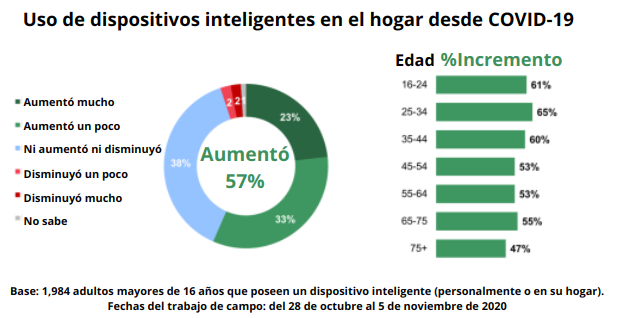
\includegraphics[width=\textwidth]{Imágenes/Uso_de_dispositivos_inteligentes_iot_covid19.png} 
    \caption{Crecimiento del uso de dispositivos inteligentes IoT}
    \label{tab:uso_dispositivos_iot}
\end{table}

\begin{table}[ht]
    \centering
        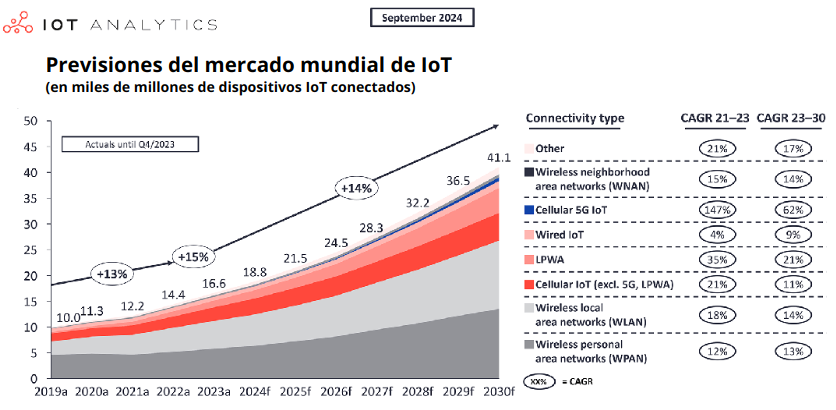
\includegraphics[width=\textwidth]{Imágenes/analytics_IoT_2024.png}
    \caption{IoT 2019-2030}
    \label{tab:iot_analytics}
\end{table}

\begin{table}[ht]
    \centering
        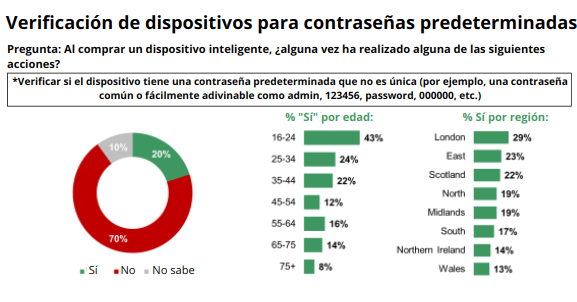
\includegraphics[width=\textwidth]{Imágenes/verificacion_.png}
    \caption{Verificación de dispositivos para contraseñas predeterminadas}
    \label{tab:verificacion_de_dispositivos_para_contraseñas_predeterminadas}
\end{table}


La información proporcionada en los cuadros \ref{tab:uso_dispositivos_iot}, \ref{tab:iot_analytics} y \ref{tab:verificacion_de_dispositivos_para_contraseñas_predeterminadas} brinda herramientas para comprender el crecimiento en el uso y adopción de las tecnologías, así como también los comportamientos de los consumidores en relación con la seguridad del IoT. La inclusión de estos informes pretende proporcionar un marco contextual que resalte la importancia de la seguridad en el desarrollo y adopción de IoT, ofreciendo una perspectiva basada en datos empíricos recolectados directamente de los usuarios finales. \cite{ipsos2021iot} \cite{Sinha2023}

La expansión del ecosistema IoT ha generado el interés de los ciberdelincuentes por sus brechas de seguridad, convirtiéndolo en un mercado fácil y atractivo para explotar. Un informe reciente de la empresa de seguridad Check Point destaca un incremento preocupante en la cantidad de ciberataques dirigidos a dispositivos IoT por sectores.\cite{checkpoint2023iot}. Por su parte la empresa Verizon también reporta incrementos con respecto del año 2023 a 2024, sumando en este último año los ataques a la cadena de suministro en sus estadísticas. Esto quiere decir que los ataques han crecido no sólo en número, sino también en sofisticación \cite{Verizon2023} \cite{Verizon2024} 

\begin{table}[ht]
    \centering
        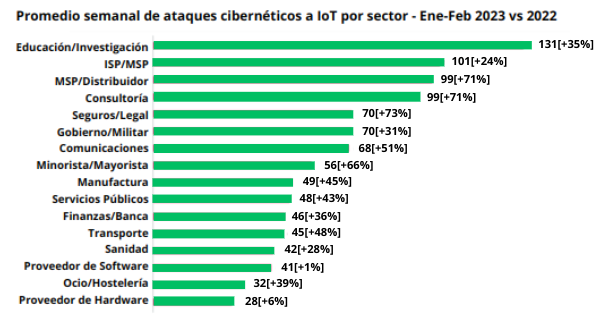
\includegraphics[width=\textwidth]{Imágenes/Promedio_semanal_de_ataques_IoT_2023vs2022.png} 
    \caption{Promedio semanal de ataques IoT 2023 vs 2022 - Check Point}
    \label{tab:promedio_semanal_de_ataques_IoT_2023vs2022}
\end{table}

El incremento en la adopción de dispositivos IoT fue más notorio desde la pandemia COVID-19 y podría creerse que las vulnerabilidades en las tecnologías comenzaron allí, pero esto no es cierto. Las brechas de seguridad vienen de tiempo atrás. Por este motivo quiero citar el trabajo de campo que realizó el Lic. Ricardo Brea, en el cual desarrolló un software integrador homogéneo y seguro para IoT culminado en 2017. Dentro de su investigación se encuentran las brechas acerca de privacidad, contemplando que en Argentina el uso de los datos está regulado por la ley de protección de datos personales (Ley 25.326), pero la jurisprudencia no se adelanta a la tecnología, si no que actúa como consecuencia de ella, y por lo tanto queda desactualizada frente nuevas tecnologías. Destaca también que los dispositivos IoT son susceptibles a ataques cibernéticos al no enviar la información encriptada, lo cual es un riesgo grave teniendo en cuenta que recolectan información de la vida de las personas y algunos poseen actuadores que encienden diversos elementos. Esto significa que un ataque cibernético a un dispositivo IoT puede causar no sólo la perdida de información, sino también una perdida material, o en el peor de los casos causar la muerte si el dispositivo atacado es un elemento que monitorea los signos vitales de una persona enferma. Un caso especial en la seguridad de IoT es cuando un dispositivo es infiltrado y utilizado, sin el conocimiento del usuario, para atacar a un tercero. IoT se convierte en un blanco ideal de ataques informáticos por la gran cantidad de dispositivos que pueden ser “reclutados” a fin de infiltrar y “reclutar” dispositivos para un ataque de denegación de servicio. Este trabajo fue presentado en el XXIV Congreso Argentino de Ciencias de la Computación (CACIC 2018)\cite{brea2018hub}

Las soluciones que existían en 2017/2018 para el uso de IoT no se encontraban integradas, eran inseguras o no eran transparentes en el manejo de la información. En la actualidad transitando el 2024, estas problemáticas siguen vigentes. 

Dentro de la presente investigación, se examinó el artículo ''Regulación mediante "bricking": ordenamiento privado en IoT''\cite{Tusikov2019} , el cual se refiere al deterioro o destrucción deliberada del software con la intención de afectar negativamente la funcionalidad del producto. El artículo argumenta y sostiene que se está empleando bricking a través de la regulación post-compra de bienes conectados a Internet, y que las empresas del “Internet de las Cosas” (IoT) tienen una capacidad injusta para imponer sus políticas preferidas de manera unilateral, automática y remota. Induciendo que el control sobre el software permite por tanto, el control sobre el hardware.

Las brechas de seguridad van dejado el paso abierto a que se consoliden diferentes vulnerabilidades. La empresa líder proveedora de soluciones de seguridad Sectigo, informa la batalla entre los ciberataques y las tecnologías de seguridad.(Cuadro: \ref{tab:evolucion_de_los_ciberataques}), evidenciando el incremento y recurrencia de las Botnets. Según Sectigo la evolución de los ataques a dispositivos IoT se puede dividir en tres eras.(Figura: \ref{fig:sectigo_eras_de_evolucion}).\cite{SectigoNoDate}

\begin{table}[ht]
    \centering
        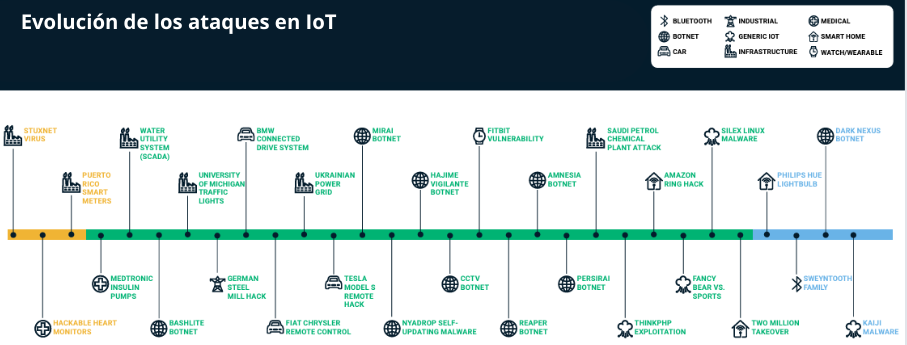
\includegraphics[width=\textwidth]{Imágenes/evolution_of_attacks_iot_sectigo..png} 
    \caption{Evolución de los ciberataques}
    \label{tab:evolucion_de_los_ciberataques}
\end{table}

\begin{figure}[ht]
    \centering
    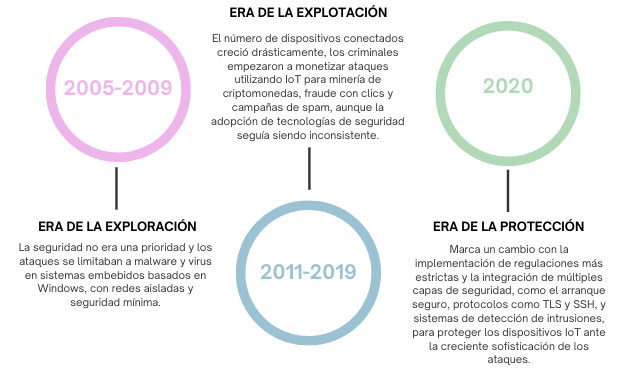
\includegraphics[width=\textwidth]{Imágenes/sectigo_eras_de_evolucion.png}
    \caption{Eras de la evolución de los ciberataques por Sectigo}
    \label{fig:sectigo_eras_de_evolucion}
\end{figure}

Al realizar esta tesis surgió la necesidad de conocer las normativas, regulaciones y entidades existentes para los heterogéneos dispositivos IoT. Dentro de las entidades gubernamentales que defienden el derecho de los consumidores, y reflejan esta defensa en regulaciones se encuentra el ''GDPR'' (General Data Protection Regulation) perteneciente al consejo de la UE(Union Europea), considerada la ley de privacidad y seguridad más estricta del mundo.\cite{consilium_data_protection}

\begin{wrapfigure}{r}{0.35\textwidth} %this figure will be at the right
    \centering
    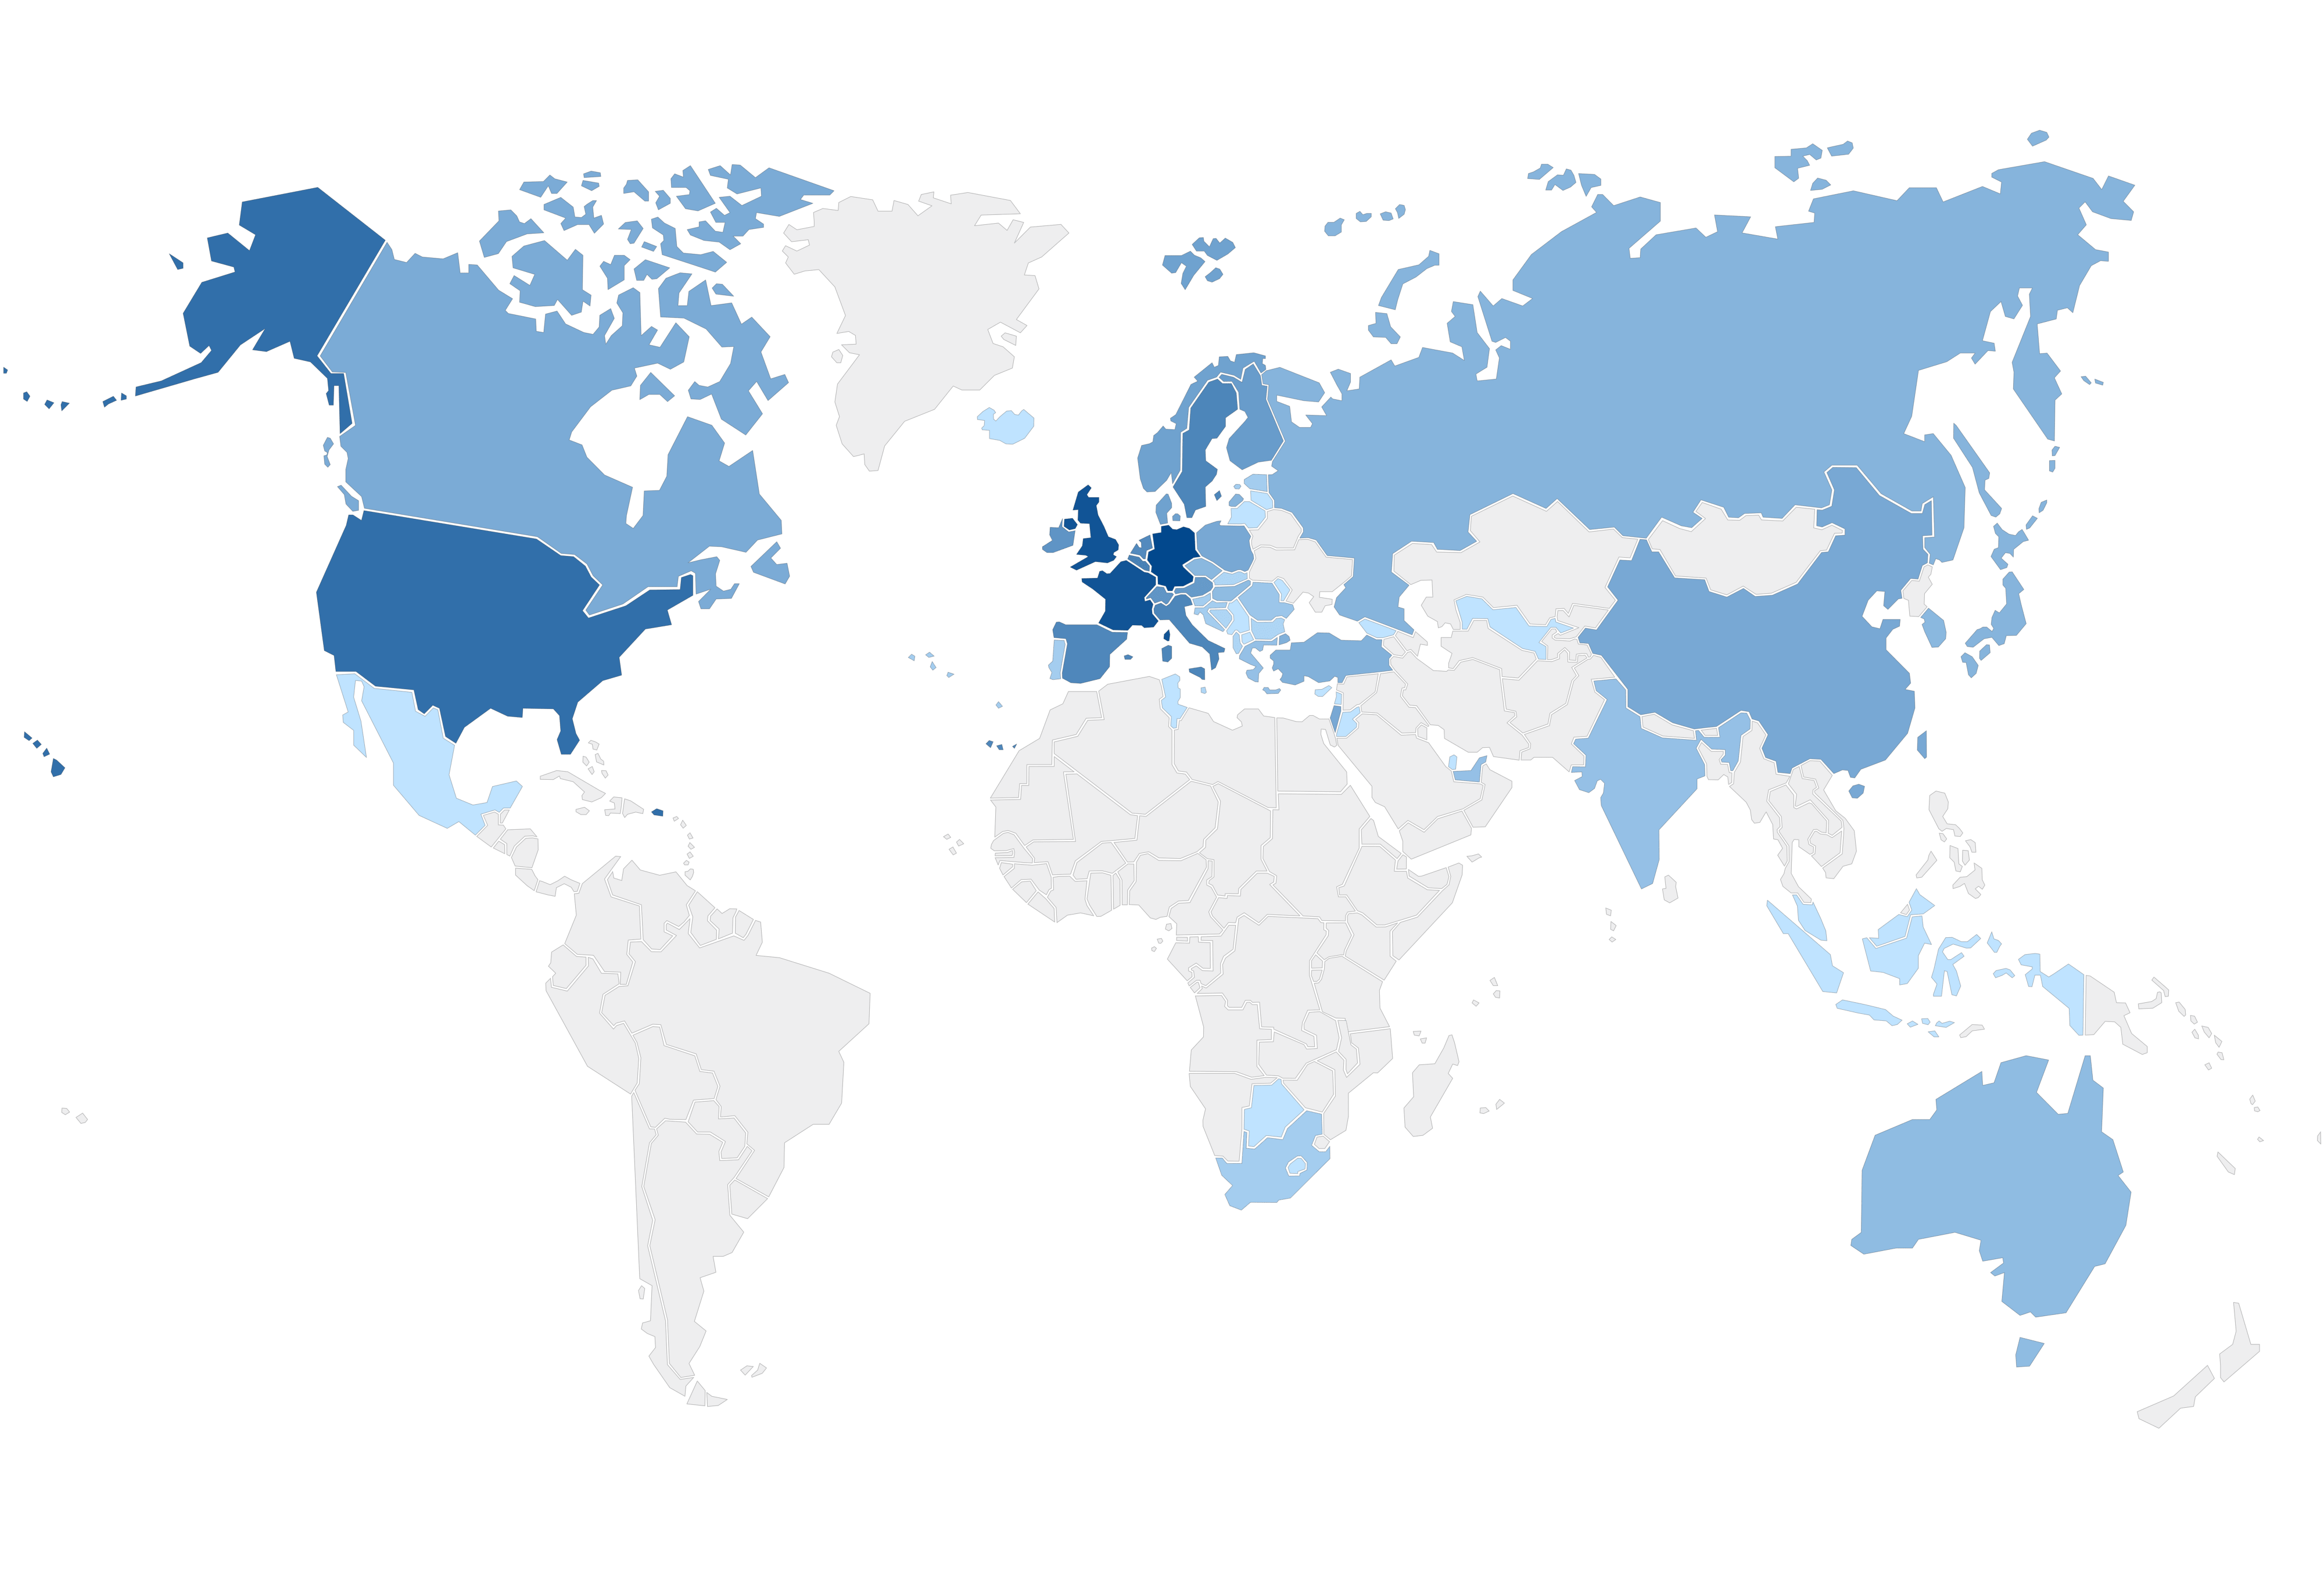
\includegraphics[width=0.35\textwidth]{Imágenes/world-mapETSI.png}
      \caption{Mapa ETSI}
    \label{fig:world-map}
\end{wrapfigure}

El reglamento GDPR actualizó y modernizó la directiva de protección de datos de 1995, fue adoptado en 2016 y entró en vigor el 25 de mayo de 2018, definiendo los derechos fundamentales de los individuos en la era digital, las obligaciones de quienes tratan los datos, los métodos para garantizar el cumplimiento y las sanciones para quienes incumplan las normas. Sin embargo, no cubre todas las particularidades de IoT, es por ello que el ''ETSI'' (European Telecommunications Standards Institute) es el organismo reconocido de normalización regional que se ocupa de las telecomunicaciones, la radiodifusión y otras redes y servicios de comunicaciones electrónicas, con más de 850 organizaciones miembros, que provienen de más de 60 países y cinco continentes.(Figura:\ref{fig:world-map})


ETSI brinda desde el año 2020 un estándar para dispositivos conectados, su objetivo es establecer disposiciones de alto nivel para la seguridad y protección de datos en dispositivos IoT, proporcionando directrices concisas para organizaciones involucradas en el desarrollo y/o fabricación de dispositivos IoT de consumo, indicando cómo implementar las disposiciones de seguridad establecidas.\cite{ETSI_EN303645_2020}.(Cuadro: \ref{tab:resumen_ETSI_directrices})

\begin{table}[ht]
    \centering
        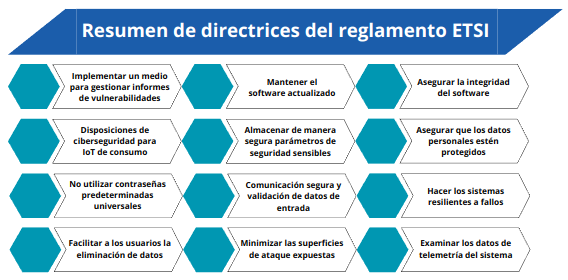
\includegraphics[width=\textwidth]{Imágenes/resumen_directrices_ETSI.png} 
    \caption{Directrices de requerimientos básicos definidos por ETSI 2020}
    \label{tab:resumen_ETSI_directrices}
\end{table}

\begin{wrapfigure}{r}{0.50\textwidth} %this figure will be at the right
   \centering
    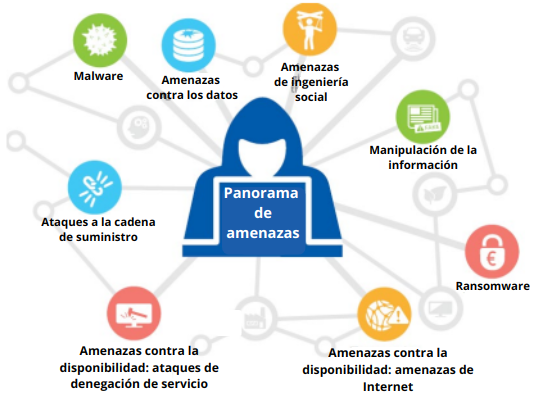
\includegraphics[width=0.50\textwidth]{Imágenes/enisa_panorama_de_amenazas_informe_2023.png}
    \caption{Informe anual ENISA 2023}
    \label{fig:informe-Panorama-de-amenazas-ENISA}
\end{wrapfigure}

La agencia ENISA(European Union Agency for Cybersecurity) es otra organización que colabora en mejorar la ciberseguridad en los estados miembros de la UE y fortalecer la capacidad de respuesta ante incidentes. En su informe anual más reciente sobre el panorama de amenazas de ciberseguridad ENISA identifica las principales amenazas, tendencias, actores maliciosos, técnicas de ataque, analizando su impacto y motivaciones e incluyendo recomendaciones sobre medidas de mitigación.\cite{enisa2023}


Dentro de las organizaciones más relevantes en cuanto a las amenazas y vulnerabilidades se encuentra OWASP(Open Worldwide Application Security Project) una fundación sin fines de lucro que trabaja en mejorar la seguridad en el software. 

OWASP Publica un ranking de las 10 vulnerabilidades más comunes de software que es referenciada en muchos análisis de seguridad.\cite{owaspTopTen}, Así como también enumera y explica, las vulnerabilidades más comunes halladas en los dispositivos IoT.\cite{owasp}

\begin{figure}[ht]
    \centering
    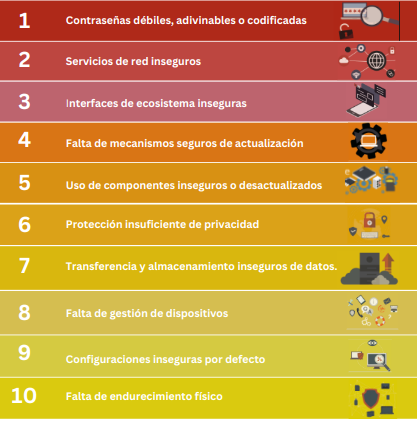
\includegraphics[width=0.7\textwidth]{Imágenes/OWASP_top_10.png}
    \caption{Resumen OWASP 2018 IoT Top10}
    \label{fig:OWASP_2018_IoT_Top10}
\end{figure}

Dado que las regulaciones GDPR y ETSI datan de algunos años atrás se investigó acerca de la actualidad para conocer si han surgido nuevas soluciones a las problemáticas de IoT. Existe un trabajo de investigación y práctica que implementa SecOps realizado en 2023 abordando los desafíos mediante técnicas combinadas de seguridad, operaciones y buenas prácticas. Este trabajo da muestras de las mejoras y mitigaciones que se pueden lograr en dispositivos ya existentes si se aplican las medidas necesarias. Si bien, los desafíos eran los mismos de años atrás(figura: \ref{fig:iot_challenges}), utilizar un enfoque moderno ha mejorado de manera contundente los resultados.\cite{jorgensen2023secops}

\begin{figure}[ht]
    \centering
    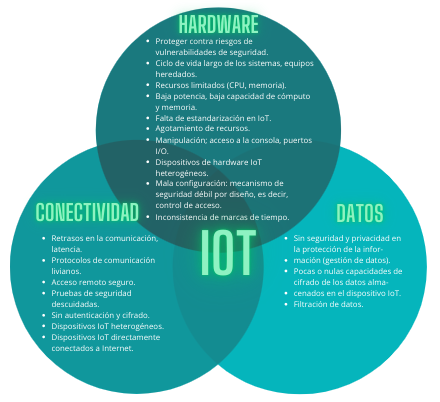
\includegraphics[width=0.9\textwidth]{Imágenes/desafios_iot_por_capas.png}
    \caption{Desafíos de seguridad existentes en 2023 para IoT}
    \label{fig:iot_challenges}
\end{figure}

La escasez de soluciones y mitigaciones tempranas a las vulnerabilidades de las tecnologías IoT, que avanzan a mayor velocidad que las medidas adecuadas de contención en temas referentes a la seguridad en los dispositivos de comercialización, se convierten en la motivación necesaria para realizar el presente trabajo, proponiendo la implementación de DevSecOps como medida cautelar y mitigatoria de los desafíos emergentes.
%!TEX root = ../thesis.tex
%*******************************************************************************
%****************************** Second Chapter *********************************
%*******************************************************************************
\chapter{Marco teórico}

\textbf{IoT}

La IETF (Internet Engineering Task Force) define el IoT (Internet of Things) como una red de dispositivos físicos (objetos, sensores, dispositivos electrónicos, software, etc.) que están conectados a internet y son capaces de recopilar, intercambiar y procesar datos a través de la red sin intervención humana. Estos dispositivos pueden interactuar entre sí, actuar automáticamente y ser controlados de manera remota mediante la infraestructura de internet.
Un documento clave de la IETF sobre IoT es el RFC 7452, que describe los requisitos y desafíos técnicos relacionados con la conectividad, la seguridad y la interoperabilidad de los dispositivos IoT. Se enfatiza la importancia de estándares abiertos, seguridad robusta y escalabilidad para manejar la vasta cantidad de dispositivos que estarán conectados en el futuro.
En resumen, IoT según la IETF se refiere a un ecosistema de objetos conectados y autónomos que interactúan a través de internet para realizar tareas inteligentes y automatizadas.\cite{rfc7452}

\textbf{Firmware}

El firmware es un tipo de software que proporciona instrucciones de máquina a los componentes de hardware de un dispositivo, lo que le permite funcionar a un nivel básico. Dado que el firmware lo instala el fabricante y normalmente no se puede eliminar, a veces se denomina software integrado. El firmware se encarga de la comunicación entre el sistema operativo y el hardware. En esencia, el firmware le indica a un dispositivo cómo debe funcionar a un nivel muy básico.\cite{avg2024}

Existen consideraciones de la IETF en cuanto a la implementación de firmware. Para esto, se debe utilizar la autenticación y la protección de la integridad de las imágenes de firmware, pero la protección confidencial del firmware es opcional. En el caso de las actualizaciones de firmware se realizan no sólo para corregir errores, sino también para agregar nuevas funcionalidades y reconfigurar el dispositivo para que funcione en nuevos entornos o se comporte de manera diferente en un contexto ya implementado.\cite{rfc9019}

\textbf{Convenciones, terminologías y partes interesadas del firmware}

\begin{itemize}
    \item \textbf{Imagen de firmware: } Es un binario que puede contener el software completo de un dispositivo o un subconjunto del mismo. La imagen de firmware puede constar de varias imágenes si el dispositivo contiene más de un microcontrolador. Una imagen de firmware de aplicación, como indica su nombre, contiene el programa de aplicación, que a menudo incluye todo el código necesario para ejecutarlo (como pilas de protocolos y un sistema operativo (OS) integrado).
    \item \textbf{Manifiesto:} El manifiesto contiene metadatos sobre la imagen del firmware. El manifiesto está protegido contra modificaciones y proporciona información sobre el autor.
    \item \textbf{Autor: } Es la entidad que crea la imagen del firmware. 
    \item \textbf{Operador del dispositivo: } Es responsable del funcionamiento diario de una flota de dispositivos IoT. 
    \item \textbf{Operador de red: } Es responsable del funcionamiento de una red a la que se conectan los dispositivos IoT.
    \item \textbf{Rastreador de estado: } El rastreador de estado tiene un componente cliente y un componente servidor y realiza tres tareas:
    \begin{enumerate}
    \item Comunica la disponibilidad de una nueva versión de firmware. Esta información fluirá del servidor al cliente.
    \item Transmite información sobre las características del software y hardware del dispositivo. El flujo de información va del cliente al servidor.
    \item Puede activar de forma remota el proceso de actualización del firmware. El flujo de información va del servidor al cliente.
    \end{enumerate}
    
    \item \textbf{Consumidor de firmware: } Es el destinatario de la imagen de firmware y del manifiesto. Es responsable de analizar y verificar el manifiesto recibido y de almacenar la imagen de firmware obtenida. Interactúa con el servidor de firmware y el cliente de seguimiento de estado (localmente).
    
    \item \textbf{Servidor de firmware: } Almacena imágenes de firmware y manifiesto. Distribuye a los dispositivos IoT.
    \item \textbf{Cargador de arranque: } Un gestor de arranque es un programa que se ejecuta una vez que se reinicia un microcontrolador. Es el encargado de decidir qué código ejecutar.
\item \textbf{Dispositivo (IoT): } Se refiere a todo el producto de IoT, que consta de uno o varios microcontroladores, sensores y/o actuadores. Muchos de los dispositivos de IoT que se venden hoy en día contienen varios microcontroladores; por lo tanto, un solo dispositivo puede necesitar obtener más de una imagen y manifiesto de firmware para realizar una actualización correctamente.\cite{rfc9019}

La IETF a través del RFC 7228.\cite{rfc7228}, clasifica los dispositivos de IoT en tres clases principales basadas en sus limitaciones de recursos:

    \begin{itemize}
        \item \textbf{Clase 0: }Dispositivos extremadamente restringidos. Tienen capacidades de procesamiento y memoria muy limitadas, lo que les impide manejar comunicaciones seguras directamente con Internet. Generalmente, dependen de puertas de enlace o servidores proxy para la comunicación.
        \item \textbf{Clase 1: }Estos dispositivos son un poco más potentes que los de C0, pero aún limitados. Pueden manejar protocolos ligeros como CoAP y DTLS para la comunicación segura, pero no son capaces de utilizar protocolos más complejos como HTTP o TLS sin asistencia de una puerta de enlace.
        \item \textbf{Clase 2: }Dispositivos con muchas menos restricciones, similares a los teléfonos móviles o portátiles en términos de capacidades de procesamiento. Son capaces de manejar protocolos más robustos y completos sin necesidad de intermediarios, y tienen un mayor potencial para interoperabilidad y soporte de aplicaciones complejas.
    \end{itemize}

\begin{table}[ht]
    \centering
    \begin{tabular}{|>{\centering\arraybackslash}p{4cm}|>{\centering\arraybackslash}p{4cm}|>{\centering\arraybackslash}p{4cm}|}
        \hline
        \textbf{Nombre} & \textbf{Tamaño de datos} \newline \textbf{(Ej. RAM)} & \textbf{Tamaño de código} \newline \textbf{(Ej. Flash)}\\
        \hline
        \textbf{Clase 0 (C0)}  & $\ll$ 10 KiB   & $\ll$ 100 KiB \\
        \textbf{Clase 1 (C1)}  & $\sim$ 10 KiB  & $\sim$ 100 KiB \\
        \textbf{Clase 2 (C2)}  & $\sim$ 50 KiB  & $\sim$ 250 KiB \\
        \hline
    \end{tabular}
    \caption{Clases de dispositivos restringidos (KiB = 1024 bytes)}
    \label{tab:Clases_de_dispositivos_restringidos}
\end{table}

\end{itemize}

Para visualizar de qué manera opera e interactúan los componentes y la arquitectura se ha tomado el modelo de la IETF(Figura \ref{fig:arquitectura_de_firmware}).\cite{rfc9019}

\begin{figure} [ht]
    \centering
     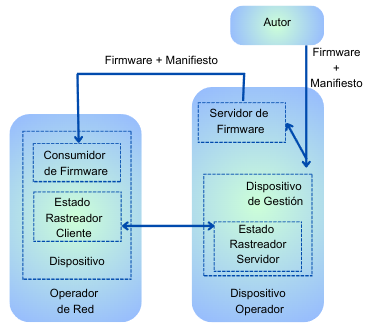
\includegraphics[width=0.6\textwidth]{Imágenes/arquitectura_firmware.png}
    \caption{Arquitectura de firmware}
    \label{fig:arquitectura_de_firmware}
\end{figure}

\newpage

\textbf{Protocolos de red y comunicación}

El protocolo de comunicación determinara la seguridad, usabilidad y robustez de la solución porque es el centro de la misma.

La comunicación en IoT es cliente servidor donde un cliente puede ser un dispositivo con capacidad de conexión a Ethernet o un Gateway y un servidor puede ser un servicio en la nube o un Gateway local.\cite{brea2018hub}

\textbf{HTTP} 

HTTP(Hypertext Transfer Protocol), es un protocolo utilizado para la transferencia de información en la web. Permite la comunicación entre un navegador web y un servidor, facilitando la carga de páginas web y la transmisión de datos, actúa en la capa 7 del modelo OSI y utiliza el puerto 80 de manera predeterminada.

\textbf{CoAP} 

CoAP(RFC 7252 Constrained of Application Protocol) es un protocolo de transferencia web especializado para su uso con nodos restringidos y redes restringidas en la Internet de las Cosas. El protocolo está diseñado para aplicaciones de máquina a máquina (M2M), como la energía inteligente y la automatización de edificios.\cite{coap_space}

\textbf{MQTT} 

MQTT es un protocolo de transporte de mensajes de publicación/suscripción de cliente-servidor. Es liviano, abierto, simple y está diseñado para ser fácil de implementar. Estas características lo hacen ideal para su uso en muchas situaciones, incluidos entornos restringidos como la comunicación en contextos de máquina a máquina (M2M) e Internet de las cosas (IoT) donde se requiere una pequeña huella de código y/o el ancho de banda de la red es limitado.

El protocolo se ejecuta sobre TCP/IP o sobre otros protocolos de red que proporcionan conexiones ordenadas, bidireccionales y sin pérdidas. Entre sus características se incluyen:

\begin{itemize}
    \item Uso del patrón de mensajes de publicación/suscripción que proporciona distribución de mensajes de uno a muchos y disociación de aplicaciones.
    \item Un transporte de mensajería que es independiente del contenido de la carga útil.
    \item Tres calidades de servicio para la entrega de mensajes(Quality of Service):
    \begin{itemize}
        \item \textbf{Como máximo una vez}, donde los mensajes se envían según los mejores esfuerzos del entorno operativo. Puede ocurrir pérdida de mensajes. Este nivel se podría utilizar, por ejemplo, con datos de sensores ambientales donde no importa si se pierde una lectura individual ya que la siguiente se publicará poco después.\textbf{(QoS=0)}
        \item \textbf{Al menos una vez}, donde se asegura que los mensajes llegarán pero pueden aparecer duplicados.\textbf{(QoS=1)}
        \item \textbf{Exactamente una vez}, donde se garantiza que el mensaje llegará exactamente una vez. Este nivel podría utilizarse, por ejemplo, en sistemas de facturación donde los mensajes duplicados o perdidos podrían dar lugar a la aplicación de cargos incorrectos.\textbf{(QoS=2)}
    \end{itemize}
    \item Una pequeña sobrecarga de transporte y intercambios de protocolo minimizados para reducir el tráfico de red.
    \item Un mecanismo para notificar a las partes interesadas cuando ocurre una desconexión anormal.\cite{mqtt-v5.0}
\end{itemize}

La seguridad en MQTT se divide en varias capas. Cada capa previene distintos tipos de ataques. El objetivo de MQTT es proporcionar un protocolo de comunicación ligero y fácil de usar para IoT. El protocolo en sí mismo especifica sólo unos pocos mecanismos de seguridad. Las implementaciones de MQTT suelen utilizar otros estándares de seguridad de última generación: por ejemplo, SSL/TLS para la seguridad del transporte. Dado que la seguridad es difícil, tiene sentido basarse en estándares generalmente aceptados.\cite{hivemq_mqtt_security}
\begin{table}[ht]
\centering
\begin{tabular}{|l|p{10cm}|}
\hline
\textbf{Nivel} & \textbf{Descripción}  \\ \hline
\textbf{Nivel de red} & Utilizar una red físicamente segura o VPN para todas las comunicaciones entre clientes y brókers. Adecuada para aplicaciones de puerta de enlace, donde la puerta está conectada a dispositivos por un lado y con el bróker a través de VPN por el otro lado. \\ \hline
\textbf{Nivel de transporte} & TLS/SSL se utiliza para garantizar la confidencialidad y autenticación durante la transmisión. Es un método seguro y comprobado que cifra los datos y verifica las identidades mediante certificados de cliente. Ideal para comunicaciones seguras. \\ \hline
\textbf{Nivel de aplicación} & MQTT proporciona un identificador de cliente y credenciales de nombre de usuario y contraseña para autenticar dispositivos. La autorización se define en el bróker, y es posible utilizar cifrado de carga útil en este nivel para proteger los datos sin requerir cifrado de transporte. \\ \hline
\end{tabular}
\caption{Seguridad en los diferentes niveles de comunicación MQTT}
\end{table}

La seguridad de la capa de transporte (TLS) y la capa de sockets seguros (SSL) proporcionan un canal de comunicación seguro entre un cliente y un servidor. En esencia, TLS y SSL son protocolos criptográficos que utilizan un mecanismo de enlace para negociar varios parámetros y crear una conexión segura entre el cliente y el servidor. Una vez completado el enlace, se establece una comunicación cifrada entre el cliente y el servidor y ningún atacante puede espiar ninguna parte de la comunicación. Los servidores proporcionan un certificado X509 (normalmente emitido por una autoridad de confianza) que los clientes utilizan para verificar la identidad del servidor.

MQTT se basa en el protocolo de transporte TCP. De forma predeterminada, las conexiones TCP no utilizan comunicación cifrada. Para cifrar toda la comunicación MQTT, muchos agentes MQTT permiten el uso de TLS en lugar de TCP simple. El puerto 8883 está reservado exclusivamente para MQTT sobre TLS.\cite{hivemq-mqtt-security_tls_ssl}

Para proporcionar confidencialidad de comunicación y autenticación de Broker a los clientes MQTT, se utiliza TLS y se recomienda TLS 1.3\cite{rfc8446}.

El documento RFC9431\cite{rfc9431} describe los intercambios de mensajes como interacciones del protocolo MQTT. Los clientes son clientes MQTT, que se conectan al Broker para publicar y suscribirse a los mensajes de la aplicación (que están etiquetados con sus temas).

Conceptos clave en el protocolo MQTT:

\begin{itemize}
    \item \textbf{Broker: }El broker MQTT. Actúa como intermediario entre los clientes que publican mensajes de aplicación y los clientes que realizaron suscripciones. El intermediario actúa como servidor de recursos para los clientes.
    \item \textbf{Cliente: }Un dispositivo o programa que utiliza MQTT.
    \item \textbf{Conexión de red: }Una construcción proporcionada por el protocolo de transporte subyacente que utiliza MQTT. Conecta al Cliente con el Servidor. Proporciona los medios para enviar un flujo de bytes ordenado y sin pérdidas en ambas direcciones. Este documento utiliza TLS como protocolo de transporte.
    \item \textbf{Sesión: }Una interacción con estado entre un cliente y un agente. Algunas sesiones duran solo lo que dura la conexión de red; otras pueden abarcar varias conexiones de red.
    \item \textbf{Mensaje de la aplicación: }Los datos que se transmiten mediante el protocolo MQTT tienen un nivel de calidad de servicio (QoS) y un nombre de tema asociados.
    \item \textbf{Paquete de control MQTT: }El protocolo MQTT funciona intercambiando una serie de paquetes de control MQTT. Cada paquete se compone de un encabezado fijo, un encabezado variable (según el tipo de paquete de control) y una carga útil.
    \item \textbf{Cadena codificada en UTF-8: }Una cadena con un campo de dos bytes como prefijo que indica la cantidad de bytes de una cadena codificada en UTF-8. A menos que se indique lo contrario, todas las cadenas codificadas en UTF-8 pueden tener cualquier longitud en el rango de 0 a 65535 bytes.
    \item \textbf{Datos binarios: }Los datos binarios se representan mediante un campo de dos bytes de longitud, que indica la cantidad de bytes de datos, seguida de esa cantidad de bytes. Por lo tanto, la longitud de los datos binarios está limitada al rango de 0 a 65535 bytes.
    \item \textbf{Byte variable entero: }Un entero de byte variable se codifica mediante un esquema de codificación que utiliza un solo byte para valores de hasta 127. Para valores mayores, los siete bits menos significativos de cada byte codifican los datos y el bit más significativo se utiliza para indicar si hay bytes siguientes en la representación. Por lo tanto, cada byte codifica 128 valores y un "bit de continuación". La cantidad máxima de bytes en el campo Entero de byte variable es cuatro.
    \item \textbf{Propiedad: }El último campo del encabezado de variable es un conjunto de propiedades para varios paquetes de control MQTT. Una propiedad consta de un identificador que define su uso y tipo de datos, seguido de un valor. El identificador se codifica como un entero de byte variable.
    \item \textbf{Topic Name: }La etiqueta adjunta a un mensaje de aplicación, que coincide con una suscripción.
    \item \textbf{Suscripción: }Una suscripción incluye un filtro de temas y una calidad de servicio máxima. Una suscripción está asociada a una única sesión.
    \item \textbf{Filtro de temas: }Una expresión que indica interés en uno o más nombres de temas. Los filtros de temas pueden incluir comodines.
\end{itemize}


En el protocolo MQTT de publicación-suscripción, después de conectarse al MQTT Server (Broker), un Cliente puede publicar y suscribirse a múltiples temas.  El Broker, que actúa como Servidor de Recursos (RS), se encarga de distribuir los mensajes publicados por los editores a sus suscriptores.
Los mensajes se publican bajo un "Topic Name", y los suscriptores se suscriben a los Topic Names para recibir los mensajes correspondientes.  El Broker utiliza el nombre de tema de un mensaje publicado para determinar suscriptores deben recibir los mensajes. 

\begin{wrapfigure}{r}{0.45\textwidth} %this figure will be at the right
    \centering
    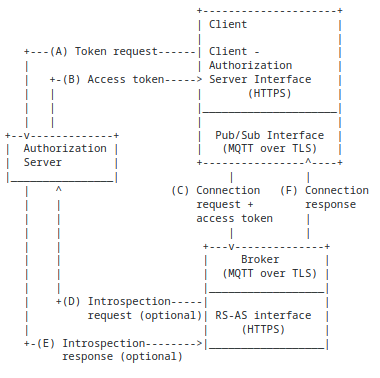
\includegraphics[width=0.45\textwidth]{Imágenes/rfc9431setup_connection.png}
    \caption{Connection setup rfc9431}
    \label{fig:setup_MQTT}
\end{wrapfigure}

Un Propietario de Recursos puede preconfigurar políticas en el Servidor de Autorización (AS) que dan a los Clientes permisos de publicación o suscripción a diferentes temas.
Los clientes demuestran su permiso para publicar y suscribirse a temas alojados en un Broker MQTT mediante un token de acceso vinculado a una clave de prueba de posesión (PoP).

Si el Cliente tiene recursos limitados o no admite HTTPS, un Servidor de Autorización de Cliente independiente puede llevar a cabo la solicitud de token en nombre del Cliente ( Figura\ref{fig:setup_MQTT} , pasos (A) y (B)) y, posteriormente, incorporar el token al Cliente.\cite{rfc9431}

\begin{figure}[ht]
    \centering
    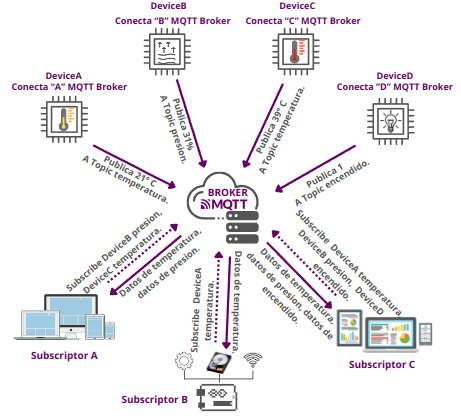
\includegraphics[width=0.86\textwidth]{Imágenes/escenario_MQTT.png}
    \caption{Escenario modelo MQTT}
    \label{fig:mqtt_escenario}
\end{figure}

\vspace{1cm}

\textbf{Tabla comparativa de protocolos}

\begin{table}[ht]
    \centering
    \begin{tabular}{|c|c|c|c|}
        \hline
        \textbf{} & \textbf{MQTTv5} & \textbf{HTTP} & \textbf{CoAP} \\
        \hline
        \textbf{Tipo} & pub/sub  & req/res & req/res \\
        \hline
        \textbf{Arquitectura} & Broker  & P2P & Broker \\
        \hline
        \textbf{Transporte} & TCP  & TCP & UDP \\
        \hline
        \textbf{Seguridad} & SSL/TLS  & SSL/TLS & DTLS \\
        \hline
        \textbf{Subscripciones} & Jerárquico por patrones & NO & Multicast \\
        \hline
        \textbf{Serialización} & Texto  & - & Configurable \\
        \hline
    \end{tabular}
    \label{tab:protocolos_comunicacion}
\end{table}


\textbf{Edge Computing/Fog Computing}

El Edge Computing, o computación en el borde, es un nuevo paradigma de computación en el que los datos del IoT son procesados en la periferia de la red (cloud edge), en la misma fuente que los genera o tan cerca de ella como sea posible. Podemos comparar el Edge Computing con los gobiernos regionales establecidos en un país para evitar que toda la gestión pase por el gobierno central o, para cerrar el símil, el Cloud Computing.\cite{Iberdrola}

\begin{figure}[ht]
    \centering
    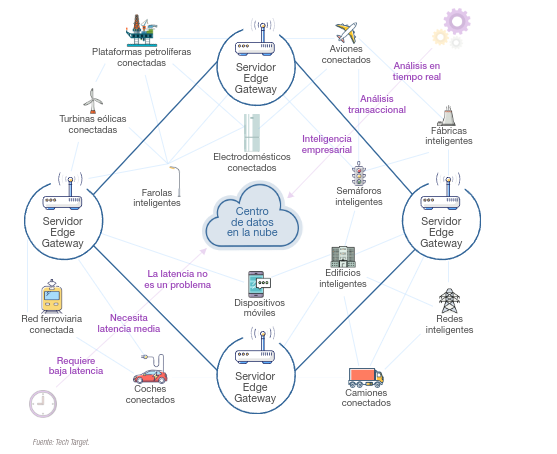
\includegraphics[width=\textwidth]{Imágenes/edge_computing.png}
    \caption{Escenario Edge Computing}
    \label{fig:edge_computing}
\end{figure}

El Edge Computing, también conocido como "Fog Computing" en algunos entornos,  es un nuevo paradigma en el que se colocan recursos de computación y almacenamiento sustanciales en el borde de Internet, cerca de  dispositivos móviles, sensores, actuadores o máquinas.Procesa tanto datos descendentes (que se originan en servicios en la nube) como datos ascendentes (que se originan en dispositivos finales o elementos de red). El término "Fog Computing" generalmente representa la noción de computación de borde de múltiples niveles, es decir, varias capas de infraestructura informática entre dispositivos finales y servicios en la nube.

Un dispositivo de borde es cualquier recurso informático o de red que reside entre las fuentes de datos de los dispositivos finales y los centros de datos basados en la nube.
En Edge Computing, los dispositivos finales consumen y producen datos.

Varias organizaciones de desarrollo de normas (Several Standards Developing Organizations) y foros de la industria han proporcionado definiciones de Edge Computing y de Fog Computing:

   * ISO define la computación de borde como una "forma de computación distribuida en qué el procesamiento y almacenamiento de datos significativos, se lleva a cabo en los nodos que están en el borde de la red".

   * ETSI define la computación de borde de acceso múltiple como un "sistema que proporciona un entorno de servicios de TI y computación en la nube. Con capacidades en el borde de una red de acceso que contiene una o más tipos de tecnología de acceso, y en estrecha proximidad a sus usuarios"

   * El Consorcio de IoT de la Industria (IIC) (que ahora incorpora lo que era anteriormente OpenFog) define el Fog Computing como "un sistema horizontal de arquitectura de niveles que distribuye la computación, el almacenamiento y el control de funciones de red más cercanas a los usuarios a lo largo de una nube a "cosa continua".

   A partir de estas definiciones, podemos resumir una filosofía general de Edge Computing como distribución de las funciones requeridas cerca de los usuarios y datos, mientras que la diferencia con los sistemas locales clásicos es el uso de funciones de gestión y orquestación adoptadas desde el Cloud Computing. \cite{RFC9556}

\begin{wrapfigure}{r}{0.40\textwidth} %this figure will be at the right
    \centering
    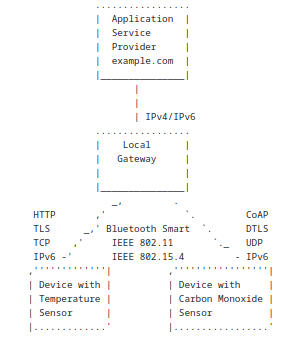
\includegraphics[width=0.40\textwidth]{Imágenes/device-to-gateway-rfc7452.png}
    \caption{Comunicación de dispositivo a Gateway}
    \label{fig:device-to-gateway-rfc7452}
\end{wrapfigure}

\textbf{Gateway}

El Gateway actúa como intermediario entre los dispositivos de IoT y los sistemas centralizados, lo que permite el procesamiento local y reduce la dependencia de los servicios en la nube para tareas urgentes o que requieren muchos datos. En dispositivos con una capacidad poca capacidad de proceso, el Gateway, agrega una capa adicional de seguridad para protegerlos de ataques.\cite{RFC9556}

Un modelo para aplicar Edge Computing en IoT es con la utilización de un elemento llamado Gateway o pasarela IoT.\cite{rfc7452}


\textbf{Supply Chain Attack}

La cadena de suministro es la secuencia de procesos involucrados en la producción de componentes, software y piezas que juntos forman un sistema, y su integración, abarcando muchas organizaciones, incluidos proveedores, vendedores y múltiples niveles de subcontratación. Es un sistema complejo, geográficamente diverso y distribuido globalmente de redes interconectadas, que cubre una amplia superficie.\cite{omitola2018}

Las cadenas de suministro de IoT son sistemas de TI vulnerables, incluidos los sistemas de IoT, que pueden verse comprometidos por ciberataques en su cadena de suministro. Los componentes comprometidos en la cadena de suministro y luego implementados en entornos operativos abren el camino a una variedad de ataques. Los ataques a la cadena de suministro son extremadamente rentables desde el punto de vista de los atacantes. Los usuarios posteriores suelen confiar implícitamente en los activos de TI que provienen de entornos de desarrollo, fabricación y distribución, a pesar de los controles de seguridad débiles o desconocidos en esos entornos. Además, un compromiso exitoso de un solo proveedor de TI bien elegido puede extenderse a toda la base de clientes del proveedor, a medida que se implementan productos y actualizaciones de software. No es coincidencia que muchos de los ciberataques más notorios hayan sido ataques a la cadena de suministro.

\begin{figure}[ht]
    \centering
    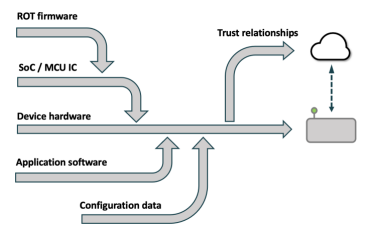
\includegraphics[width=0.5\linewidth]{Imágenes/Ramas principales de una red de suministro de dispositivos IoT típica.png}
    \caption{Supply Chain típica Iot}
    \label{fig:Supply_chain_tipoca_IoT}
\end{figure}

Esta red de suministro consta de seis tipos básicos de operaciones: diseño, que reúne los requisitos y especifica un sistema capaz de satisfacerlos; desarrollo, mediante el cual se crean y se ponen en funcionamiento activos de producción funcionales; ensamblaje de hardware, que integra progresivamente componentes y subconjuntos en dispositivos completos; programación, que instala activos lógicos en dispositivos físicos; personalización, que genera una identidad única para cada dispositivo; e integración, que coloca esos dispositivos en relaciones de confianza con otros sistemas. La programación, la personalización y la integración comprenden juntas el proceso de aprovisionamiento, mediante el cual el hardware se pone en un estado funcional.
Un ciberataque podría lanzarse en cualquier etapa de la red de suministro de un dispositivo inteligente. El diseño y el desarrollo son actividades de tipo proyecto que tienen mucho en común con los proyectos de diseño y desarrollo de software y hardware en todas partes. Durante estas fases, la seguridad es idéntica a la calidad, porque puede ser imposible distinguir entre un error y un sabotaje. Afortunadamente, existe una amplia literatura sobre ciclos de vida de desarrollo de software (SDLC) seguros y buenas prácticas de TI para proteger los entornos de desarrollo.\cite{IoTSFSCIP2022}

\textbf{Bricking}

El término 'bricking' en ciberseguridad y tecnología se refiere a un evento donde un dispositivo electrónico, como un teléfono inteligente, computadora, tableta, o cualquier dispositivo IoT, se vuelve completamente inoperable o significativamente dañado, haciéndolo tan útil como un ladrillo. Esta condición, a menudo irreversible, hace que el dispositivo no pueda realizar sus funciones primarias o encenderse, requiriendo reparaciones potencialmente costosas o reemplazos completos. El 'bricking' puede ser el resultado de actividades maliciosas deliberadas, errores graves de software o firmware, o daños accidentales durante actualizaciones o modificaciones de sistema fallidas.

El 'bricking' puede ocurrir de diversas maneras, cada una con sus mecanismos e implicaciones:
\begin{itemize}
    \item \textbf{Software Malicioso:} Malware o ataques dirigidos pueden reescribir el firmware del dispositivo o configuraciones críticas del sistema, dejando el dispositivo inoperativo.
    \item \textbf{Actualizaciones Fallidas:} Actualizaciones defectuosas o interrumpidas del firmware o sistema operativo del dispositivo pueden corromper archivos esenciales, llevando al 'bricking'.
    \item \textbf{Modificaciones No Oficiales:} Realizar 'jailbreaking' o 'rooting' con el fin de eludir las restricciones del fabricante puede exponer los dispositivos a riesgos de 'bricking', a menudo debido a modificaciones incompatibles o inestables.
    \item \textbf{Fallos de Hardware:} Aunque menos comunes, daños físicos o defectos de fabricación que afectan a componentes cruciales también pueden resultar en un estado de 'bricking'.
    \item \textbf{Ataques Remotos:} Los dispositivos conectados a internet pueden ser vulnerables a ataques remotos que explotan agujeros de seguridad para inducir 'bricking' intencionalmente, a menudo llamados ataques de "Ejecución Remota de Código" (RCE). \cite{vpnunlimited2024}
\end{itemize}
\vspace{1cm}

\textbf{DevOps}

El término DevOps, que es una combinación de los términos ingleses development(desarrollo) y operations(operaciones), designa la unión de personas, procesos y tecnología para ofrecer valor a los clientes de forma constante.

¿Qué significa DevOps para los equipos? DevOps permite que los roles que antes estaban aislados (desarrollo, operaciones de TI, ingeniería de la calidad y seguridad) se coordinen y colaboren para producir productos mejores y más confiables. Al adoptar una cultura de DevOps junto con prácticas y herramientas de DevOps, los equipos adquieren la capacidad de responder mejor a las necesidades de los clientes, aumentar la confianza en las aplicaciones que crean y alcanzar los objetivos empresariales en menos tiempo.\cite{MicrosoftDevOps}

\textbf{Procesos: }
\begin{itemize}
    \item \textbf{Integración continua y entrega continua (CI/CD): }La integración continua (CI) es la práctica que utilizan los equipos de desarrollo para la automatización, combinación y prueba de código. La integración continua ayuda a detectar errores en etapas tempranas del ciclo de desarrollo, lo que hace que sean menos costosos de corregir. Las pruebas automatizadas se ejecutan como parte del proceso de CI para garantizar la calidad. Los sistemas de CI generan artefactos y los alimentan para liberar procesos a fin de impulsar implementaciones frecuentes. La entrega continua (CD) es un proceso por el que el código se compila, prueba e implementa en uno o varios entornos de prueba y producción. La implementación y las pruebas en varios entornos aumentan la calidad. Los sistemas de CD generan artefactos que se pueden implementar, incluida la infraestructura y las aplicaciones. Los procesos de versión automatizados consumen estos artefactos para publicar versiones nuevas y correcciones en los sistemas existentes. Los sistemas que supervisan y envían alertas se ejecutan de manera continua para impulsar la visibilidad de todo el proceso de CD.
    \item \textbf{Control de versiones: }Es la práctica de administrar el código por versiones, haciendo un seguimiento de las revisiones y del historial de cambios para facilitar la revisión y la recuperación del código. Esta práctica suele implementarse con sistemas de control de versiones, como Git, que permite que varios desarrolladores colaboren para crear código. Estos sistemas proporcionan un proceso claro para fusionar mediante combinación los cambios en el código que tienen lugar en los mismos archivos, controlar los conflictos y revertir los cambios a estados anteriores. El control de versiones es también un elemento necesario en otras prácticas, como la integración continua y la infraestructura como código.
    \item \textbf{Desarrollo ágil de software: }Agile es un enfoque de desarrollo de software que resalta la colaboración en equipo, los comentarios de los clientes y los usuarios, y la alta capacidad de adaptación al cambio a través de ciclos de versión cortos. Los equipos que practican la metodología ágil proporcionan mejoras y cambios continuos a los clientes, recopilan sus comentarios y, después, aprenden y ajustan el software en función de lo que el cliente quiere y necesita. El método ágil es muy diferente a otros marcos más tradicionales, como el modelo en cascada, que incluye ciclos de lanzamiento de versiones largos definidos por fases secuenciales. Kanban y Scrum son dos marcos populares asociados al método ágil.
    \item \textbf{Infraestructura como código: }Define las topologías y los recursos del sistema de un modo descriptivo que permite a los equipos administrar esos recursos igual que lo harían con el código. Las diferentes versiones de esas definiciones se pueden almacenar en sistemas de control de versiones, donde se pueden revisar y revertir, de nuevo, igual que el código. La práctica de la infraestructura como código permite a los equipos implementar recursos del sistema de un modo confiable, repetible y controlado. Además, la infraestructura como código ayuda a automatizar la implementación y reduce el riesgo de errores humanos, especialmente en entornos complejos de gran tamaño. Esta solución repetible y confiable para la implementación de entornos permite a los equipos mantener entornos de desarrollo y pruebas que sean idénticos al entorno de producción.
    \item \textbf{Administración de configuración: }Hace referencia a la administración del estado de los recursos en un sistema, incluidos servidores, máquinas virtuales y bases de datos. El uso de herramientas de administración de la configuración permite a los equipos distribuir cambios de un modo controlado y sistemático, lo que reduce el riesgo de modificar la configuración del sistema. Los equipos utilizan herramientas de administración de la configuración para hacer un seguimiento del estado del sistema y evitar alteraciones en la configuración, que es como se desvía la configuración de un recurso del sistema a lo largo del tiempo del estado definido para él.
    \item \textbf{Supervisión continua: }Supone tener una visibilidad completa y en tiempo real del rendimiento y el estado de la totalidad de las aplicaciones. La visibilidad abarca desde la infraestructura de base que ejecuta la aplicación hasta los componentes de software de nivel superior. La visibilidad se logra mediante la recopilación de datos de telemetría y metadatos y el establecimiento de alertas para condiciones predefinidas que garanticen la atención de un operador. La telemetría incluye registros y datos de eventos recopilados de varias partes del sistema que se almacenan donde pueden analizarse y consultarse.
    \item \textbf{Planificación: }En la fase de planeamiento, los equipos de DevOps conciben, definen y describen las características y la funcionalidad de las aplicaciones y los sistemas que planean crear. Los equipos realizan el seguimiento del progreso de tareas en niveles bajos y altos de granularidad desde productos individuales a carteras de varios productos. Los equipos utilizan las siguientes prácticas de DevOps para establecer planes con agilidad y visibilidad:
         \begin{itemize}
            \item Creación de trabajo pendiente.
            \item Seguimiento de errores.
            \item Administración del desarrollo de software Agile con Scrum.
            \item Uso de paneles Kanban.
            \item Visualización del progreso con paneles.
          \end{itemize}
    \item \textbf{Desarrollo: }La fase de desarrollo comprende todos los aspectos del desarrollo de código de software. En esta fase, los equipos de DevOps llevan a cabo las tareas a continuación:
         \begin{itemize}
            \item Selección de un entorno de desarrollo.
            \item Escritura, prueba, revisión e integración del código.
            \item Compilación del código en artefactos para implementarlo en diferentes entornos.
            \item Uso de control de versiones, normalmente Git, para colaborar en el código y trabajar en paralelo.
         \end{itemize}
     Para innovar con rapidez sin sacrificar la calidad, la estabilidad ni la productividad, los equipos de DevOps:
         \begin{itemize}
            \item Utilizan herramientas altamente productivas.
            \item Automatizan los pasos cotidianos y manuales.
            \item Realizan iteraciones en incrementos pequeños mediante pruebas automatizadas e integración continua (CI).
        \end{itemize}
    \item \textbf{Entregar: }La entrega es el proceso de implementación de aplicaciones en entornos de producción de forma coherente y confiable, idealmente mediante la entrega continua (CD). En la fase de entrega, los equipos de DevOps:
        \begin{itemize}
            \item Establecen un proceso de administración de versiones con etapas de aprobación manual claras.
            \item Configuran puertas automatizadas para mover aplicaciones entre fases hasta la versión final a los clientes.
            \item Automatizan los procesos de entrega para que sean escalables, repetibles, controlados y probados correctamente.
        \end{itemize}
    La entrega también implica la implementación y configuración de la infraestructura fundamental del entorno de entrega. Los equipos de DevOps utilizan tecnologías como infraestructura como código (IaC), contenedores y microservicios a fin de ofrecer entornos de infraestructura totalmente regulados.
    \item \textbf{Operaciones: }La fase de operaciones implica el mantenimiento, la supervisión y la solución de problemas de aplicaciones en entornos de producción, que incluyen nubes híbridas o públicas como Azure. Los objetivos de los equipos de DevOps son la confiabilidad del sistema, la alta disponibilidad, la seguridad sólida y el tiempo de inactividad cero.
    La entrega automatizada y las prácticas de implementación segura ayudan a los equipos a identificar y paliar los problemas rápidamente cuando se producen. El mantenimiento de la vigilancia requiere una telemetría muy completa, alertas que permitan tomar medidas y visibilidad total de las aplicaciones y de los sistemas subyacentes.\cite{MicrosoftLearnDevOps}
\end{itemize}

\textbf{DevSecOps}

DevSecOps es una extensión de la práctica de DevOps. Cada término define diferentes funciones y responsabilidades de los equipos de software a la hora de crear aplicaciones de software.

\begin{table}[ht]
\centering
\begin{tabular}{|c|c|p{9cm}|}
\hline
\textbf{Concepto} & \textbf{Abreviatura} & \textbf{Descripción} \\ \hline
\textbf{Desarrollo} & \textbf{Dev} & Es el proceso de planificación, codificación y prueba de la aplicación. \\ \hline
\textbf{Seguridad} & \textbf{Sec} & Significa introducir elementos de seguridad en una etapa temprana del desarrollo. \\ \hline
\textbf{Operaciones} & \textbf{Ops} & Implementa, supervisa y corrige cualquier problema con el software o los dispositivos. \\ \hline
\end{tabular}
\caption{Descripción de los conceptos DevSecOps}
\end{table}

\textbf{Cultura DevSecOps}

\textbf{Comunicación:} Las empresas implementan DevSecOps pro un cambio cultural que comienza por los altos directivos. Los líderes sénior explican la importancia y los beneficios de adoptar prácticas de seguridad al equipo de DevOps. Los desarrolladores de software y los equipos de operaciones necesitan las herramientas, los sistemas y la motivación adecuados para adoptar las prácticas de DevSecOps. 

\textbf{Personas:} DevSecOps conduce a una transformación cultural que involucra a los equipos de software. Los desarrolladores de software ya no se aferran a los roles convencionales de crear, probar y desplegar el código. Al utilizar DevSecOps, los desarrolladores de software y los equipos de operaciones trabajan en estrecha colaboración con los expertos en seguridad para mejorar la seguridad en todo el proceso de desarrollo. 

\textbf{Tecnología:} Los equipos de software utilizan la tecnología para realizar pruebas de seguridad automatizadas durante el desarrollo. Los equipos de DevOps la utilizan para verificar la aplicación en busca de defectos de seguridad sin comprometer el plazo de entrega. 

\textbf{Procesamiento:} Al adoptar DevSecOps, los equipos de software realizan pruebas y evaluaciones de seguridad a lo largo de todas las fases de desarrollo. Los desarrolladores de software buscan defectos de seguridad al escribir el código. Posteriormente, un equipo de seguridad prueba la aplicación previa al lanzamiento en busca de vulnerabilidades de seguridad. Por ejemplo, podrían verificar lo siguiente:
\begin{itemize}
    \item \textbf{Autorización} para que los usuarios puedan acceder únicamente a lo que necesitan.
    \item \textbf{Validación de entradas} de modo que el software funcione correctamente al recibir datos anómalos 
\end{itemize}

El lema de DevSecOps es \textbf{“Shift-Left Security”} que significa incorporar las verificaciones de seguridad con la mayor antelación posible en el ciclo de vida de software, adaptándose a las nuevas metodologías ágiles de desarrollo.\cite{aws_devsecops}

\vspace{0.3cm}

\begin{wrapfigure}{r}{0.30\textwidth} %this figure will be at the right
    \centering
    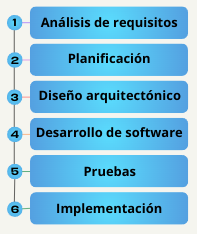
\includegraphics[width=0.25\textwidth]{Imágenes/SDLC.png}
    \caption{SDLC}
    \label{fig:Ciclo_de_vida_de_desarrollo_de_softwareSDLC}
\end{wrapfigure}

El ciclo de vida de desarrollo de software (SDLC) es un proceso estructurado que guía a los equipos de software para producir aplicaciones de alta calidad. Los equipos de software utilizan el SDLC para reducir los costos, minimizar los errores y garantizar que el software se alinee con los objetivos del proyecto en todo momento. En los métodos de desarrollo de software convencionales, las pruebas de seguridad eran un proceso independiente del SDLC, el equipo de seguridad descubre fallas sólo después de crear el software. DevSecOps mejora el SDLC mediante la detección de vulnerabilidades a lo largo del proceso de desarrollo.

\vspace{1cm}

\textbf{Componentes de DevSecOps}

\begin{itemize}
    \item \textbf{Análisis de código:} El análisis del código se refiere al proceso de investigar el código fuente de una aplicación en busca de vulnerabilidades y garantizar que se ajusta a las prácticas recomendadas de seguridad.
    \item \textbf{Administración de cambios:} Los equipos de software utilizan herramientas de administración de cambios para realizar un seguimiento de los cambios relacionados con el software o los requisitos, así como para administrarlos e informar sobre estos, evitando vulnerabilidades de seguridad involuntarias ocasionadas por los cambios en el software.
    \item \textbf{Administración del cumplimiento:} Los equipos de software se encargan de garantizar que el software cumpla con los requisitos regulatorios.
    \item \textbf{Modelado de amenazas:} Los equipos de DevSecOps investigan los problemas de seguridad que puedan surgir antes y después de desplegar la aplicación. Corrigen cualquier problema conocido y lanzan una versión actualizada de la aplicación.
    \item \textbf{Formación en seguridad:} La formación en materia de seguridad implica capacitar a los desarrolladores de software y a los equipos de operaciones en cuanto a las directrices de seguridad más recientes. De este modo, los equipos de desarrollo y de operaciones pueden tomar decisiones de seguridad independientes a la hora de crear y desplegar la aplicación.
\end{itemize}

\begin{figure}[ht]
    \centering
    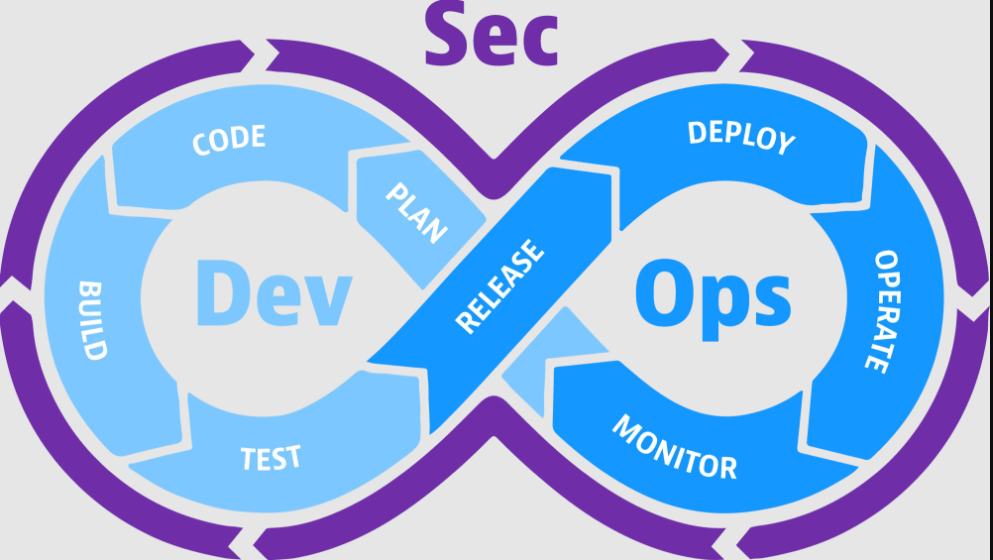
\includegraphics[width=0.75\linewidth]{Imágenes/devsecops_.png}
    \caption{Ciclo DevSecOps}
    \label{fig:enter-label}
\end{figure}

\textbf{Herramientas de DevSecOps}

\textbf{En este punto tengo una duda si lo explico asi:\href{https://ranjaniitian.medium.com/ensuring-robust-application-security-exploring-sast-dast-and-iast-for-comprehensive-protection-d68b4cf5cf79}{CLICKEA-ESTE-LINK}}

\textbf{O lo dejo como esta.........El link de arriba tiene ejemplos pero va a quedar medio largo, escucho ofertas de mediación}


\begin{table}[ht]
\centering
\begin{tabular}{|m{3cm}|m{11.5cm}|}
\hline
\centering \textbf{Concepto} & \textbf{Descripción} \\ \hline
\centering \textbf{SAST} & Las herramientas de pruebas de seguridad de aplicaciones estáticas (Static Application Security Testing) analizan y encuentran vulnerabilidades en el código fuente propio. \\ \hline
\centering \textbf{SCA} & El análisis de la composición del software (Software Composition Application) es el proceso mediante el cual se automatiza la visibilidad del uso del software de código abierto (OSS) con el fin de gestionar los riesgos, la seguridad y el cumplimiento de los requisitos de las licencias. \\ \hline
\centering \textbf{IAST} & Los equipos de DevSecOps utilizan herramientas de pruebas de seguridad de aplicaciones interactivas (Interactive Application Security Testing) para evaluar las posibles vulnerabilidades de una aplicación en el entorno de producción. IAST comprende monitores de seguridad especiales que se ejecutan desde el interior de la aplicación. \\ \hline
\centering \textbf{DAST} & Las herramientas de pruebas de seguridad de aplicaciones dinámicas (Dynamic Application Security Testing) imitan a los hackers al probar la seguridad de la aplicación desde fuera de la red. \\ \hline
\end{tabular}
\caption{Descripción de los conceptos SAST, SCA, IAST y DAST}
\end{table}


\begin{figure}[ht]
    \centering
    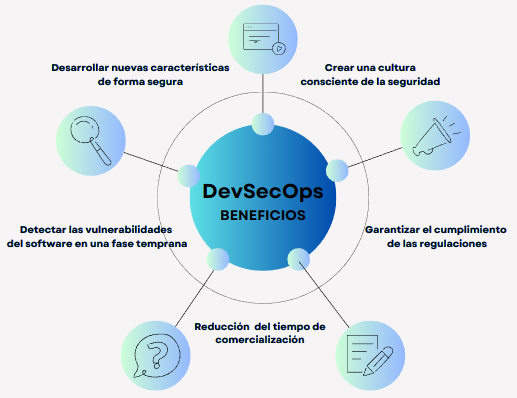
\includegraphics[width=\textwidth]{Imágenes/DevSecOps_beneficios.png}
    \caption{Beneficios DevSecOps}
    \label{fig:beneficiosdevsecops}
\end{figure}

Las pruebas de seguridad no concluyen después de que la aplicación se ponga en marcha. El equipo de operaciones no deja de supervisar para detectar posibles problemas, realizar modificaciones y trabajar con los equipos de seguridad y desarrollo para lanzar versiones actualizadas de la aplicación.


\begin{figure}[ht]
    \centering
    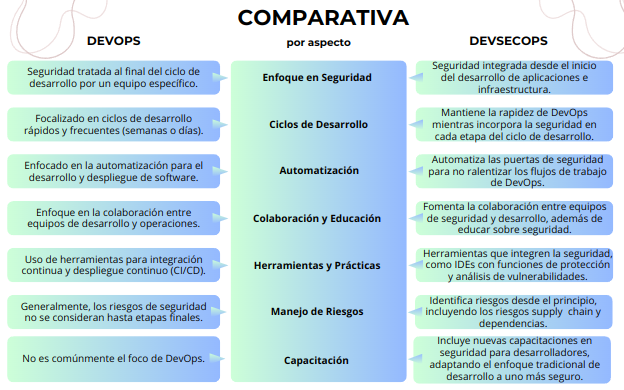
\includegraphics[width=1\linewidth]{Imágenes/comparativa_metodologias_devops_devsecops.png}
    \caption{Comparación entre DevOps y DevSecOps}
    \label{fig:comparativa_metodologias_devops_devsecops}
\end{figure}

%!TEX root = ../thesis.tex
%*******************************************************************************
%****************************** Third Chapter **********************************
%*******************************************************************************
\chapter{Desarrollo}
\label{Desarrollo}

% **************************** Define Graphics Path **************************
% \ifpdf
%    \graphicspath{{Chapter3/Figs/Raster/}{Chapter3/Figs/PDF/}{Chapter3/Figs/}}
%\else
%    \graphicspath{{Chapter3/Figs/Vector/}{Chapter3/Figs/}}
%\fi

En este capítulo se presenta la forma en la que se realizaron los experimentos y se muestran los resultados obtenidos. 


\label{Anexo}
\textbf{Procedimiento Desarrollo Seguro del Sistema}

Creo que esto va a integrarse en el desarrollo.

\textbf{Objetivo}

Asegurar el desarrollo seguro del producto de software, considerando el acceso físico y lógico no autorizado, las actualizaciones, la conexión a internet, el gateway, el sistema operativo, la dockerización, el tipo de dispositivos y el particionado de la memoria.

\textbf{Responsables:}

Desarrolladores

Administradores de Sistemas

Equipo de Seguridad Informática

\textbf{1. Accesos Lógicos No Autorizados}

\textbf{1.1. Gestión de Cuentas de Usuario:}

Establecer políticas para la creación y gestión de cuentas de usuario.

Aplicar el principio de privilegios mínimos.

\textbf{1.2. Monitoreo de Logs:}

Implementar un sistema de monitoreo de logs para detectar patrones de acceso no autorizado.

Analizar regularmente los logs para identificar posibles amenazas.

\textbf{2. Actualizaciones}

\textbf{2.1. Política de Actualizaciones:}

Establecer una política clara para la aplicación de actualizaciones de software y parches. 

Realizar actualizaciones periódicas y evaluar la necesidad de actualizaciones críticas.

\textbf{2.2. Pruebas Post-Actualización:}

Realizar pruebas exhaustivas después de cada actualización para asegurar la estabilidad del sistema.

\textbf{3. Conexión a Internet y Gateway}

\textbf{3.1. Firewalls y Filtros:}

Configurar firewalls para controlar el tráfico de red.

Utilizar filtros para bloquear tráfico malicioso.

\textbf{3.2. VPN Segura:}

Establecer conexiones a través de VPN seguras para proteger la comunicación entre sistemas.

\textbf{4. Sistema Operativo}

\textbf{4.1. Selección Segura del Sistema Operativo:}

Evaluar y seleccionar un sistema operativo que cumpla con los estándares de seguridad.

\textbf{5. Dockerización}

\textbf{5.1. Configuración Segura de Contenedores:}

Configurar los contenedores Docker con medidas de seguridad, como aislamiento de recursos.

\textbf{6. Tipo de Dispositivos}

\textbf{6.1. Evaluación de Dispositivos:}

Evaluar la seguridad de los dispositivos utilizados en el desarrollo.

Implementar políticas de uso seguro de dispositivos móviles.

\textbf{7. Particionado de la Memoria}

\textbf{7.1. Optimización y Particionado:}

Realizar un particionado adecuado de la memoria de los dispositivos para evitar vulnerabilidades.

Optimizar la asignación de recursos para mejorar el rendimiento y la seguridad.

\textbf{8. Revisiones y Actualizaciones del Procedimiento}

\textbf{8.1 Revisiones periódicas}

Revisar periódicamente el procedimiento para asegurar su relevancia y eficacia.

Actualizar el procedimiento según las cambiantes necesidades de seguridad.

\textbf{9. Acceso Físico No Autorizado}

\textbf{9.1. Control de Acceso Físico:}

Limitar el acceso físico a los servidores y equipos de desarrollo.

\textbf{9.2. Registro de Accesos:}

Mantener un registro de las personas autorizadas que ingresan a las áreas de desarrollo.

Revisar regularmente los registros para identificar cualquier acceso no autorizado.

\chapter{Conclusiones y Trabajos Futuros}
\label{conclusiones}
%Escribir:
%1- Pequeño resumen de lo realizado en el trabajo.
%2- El mejor resultado
%3- Discusión sobre los parámetros usados
%4- Trabajos futuros

\include{Chapter6/chapter6}
%\include{Chapter7/chapter7}



% ********************************** Back Matter *******************************
% Backmatter should be commented out, if you are using appendices after References
%\backmatter

% ********************************** Bibliography ******************************
\begin{spacing}{0.9}

% To use the conventional natbib style referencing
% Bibliography style previews: http://nodonn.tipido.net/bibstyle.php
% Reference styles: http://sites.stat.psu.edu/~surajit/present/bib.htm

\bibliographystyle{apalike}
%\bibliographystyle{unsrt} % Use for unsorted references  
%\bibliographystyle{plainnat} % use this to have URLs listed in References
\cleardoublepage
\bibliography{references} % Path to your References.bib file


% If you would like to use BibLaTeX for your references, pass `custombib' as
% an option in the document class. The location of 'reference.bib' should be
% specified in the preamble.tex file in the custombib section.
% Comment out the lines related to natbib above and uncomment the following line.

%\printbibliography[heading=bibintoc, title={References}]


\end{spacing}

% ********************************** Appendices ********************************

\begin{appendices} % Using appendices environment for more functunality

\include{Appendix1/appendix1}

\end{appendices}

% *************************************** Index ********************************
\printthesisindex % If index is present

\end{document}
